%%%%%%%%%% *** The Title %%%%%%%%%%
\title[]{대기광학\\\small{제16장}}

\begin{frame}[plain] %title page
	\titlepage
\end{frame}


\section{빛과 매질의 상호작용}


\begin{frame}[t]{반사}
	\begin{tabular}{ll}
		\begin{minipage}[t]{0.6\textwidth}\scriptsize
			\begin{figure}[t]
				\includegraphics[trim=50 35 350 600, clip, 
				page=479, width=\textwidth]{\bookfile}
			\end{figure}
		\end{minipage}	
		&
		\begin{minipage}[t]{0.35\textwidth} \scriptsize	
			빛이 물체와 충돌하면 일부의 빛은 표면 밖으로 전달되어 표면으로부터 후방으로 되돌려진다. \\
			이런 빛을 반사되었다고 한다. \\
			거울에서 우리의 모습을 볼 수 있게 하는 것은 반사된 빛이다. \\

			\questionset {반사의 법칙을 설명하시오.}
			\solutionset {입사각의 크기와 반사각의 크기가 같다.\\
					- 입사각: 입사하는 광선이 반사면과 수직을 이루는 법선과 이루는 각\\
					- 반사각: 반사되는 광선이 법선과 이루는 각
					}
		\end{minipage}
	\end{tabular}
\end{frame}

\begin{frame}[t]{정반사와 난반사}
	\begin{tabular}{ll}
		\begin{minipage}[t]{0.55\textwidth}\scriptsize
			\begin{figure}[t]
				\includegraphics[trim=335 430 50 120, clip, 
				page=479, width=\textwidth]{\bookfile}
			\end{figure}
		\end{minipage}	
		&
		\begin{minipage}[t]{0.4\textwidth} \scriptsize	
			표면이 매끄럽게 보인다고 하더라도 빛을 모든 방향으로 분산시키기에 충분할 정도로 실제 표면은 거칠다. \\
			이러한 반사는 유인물을 거의 모든 방향에서 읽을 수 있게 한다. 즉, 우리 주변의 대다수의 물체는 난반사에 의해 보인다. \\

			\questionset {난반사(diffuse reflection)를 설명하시오.}
			\solutionset {
					표면이 매끄럽지 않은 경우 빛이 각기 다른 각도로 입사, 반사하게 되는데 이를 난반사라고 한다. 			
					}
		\end{minipage}
	\end{tabular}
\end{frame}

\begin{frame}[t]{다중반사}
	\begin{tabular}{ll}
		\begin{minipage}[t]{0.5\textwidth}\scriptsize
			\begin{figure}[t]
				\includegraphics[trim=0 380 200 0, clip, 
				page=480, width=\textwidth]{\bookfile}
			\end{figure}
		\end{minipage}	
		&
		\begin{minipage}[t]{0.45\textwidth} \scriptsize	
			빛이 거친 표면에서 반사될 때 우리가 보는 상(image)은 보통 왜곡된 것이거나 일부 경우에는 여러 개의 상으로 보인다. \\
			거친 바다 표면에서 반사된 태양의 상은 원형이 아니라 길고 좁은 띠 형태. \\
			이는 수면의 각 파에 부딪히는 태양 빛의 일부가 관찰자의 눈을 향하여 반사되기 때문에 바다 표면에서 다중으로 왜곡되어 보인다.
		\end{minipage}
	\end{tabular}
\end{frame}

\begin{frame}[t]{내부 반사(internal reflection)}
	\begin{tabular}{ll}
		\begin{minipage}[t]{0.6\textwidth}\scriptsize
			\begin{figure}[t]
				\includegraphics[trim=270 0 0 440, clip, 
				page=480, width=\textwidth]{\bookfile}
			\end{figure}
		\end{minipage}	
		&
		\begin{minipage}[t]{0.35\textwidth} \scriptsize	
			두 소녀 위에 나타나는 반사를 주목하자. 내부 반사들은 수면과 수면 위 공기 사이의 경계에서 반사되는 빛에 의해 발생함\\

			\questionset {내부 반사를 설명하시오.}
			\solutionset {
				빛이 투명한 물체를 통하여 진행할 때, 빛이 물체의 맞은편 경계(표면)에서 투명한 물체 안으로 다시 반사되는 경우
					}

		\end{minipage}
	\end{tabular}
\end{frame}


\begin{frame}[t]{굴절(refraction)}
	\begin{tabular}{ll}
		\begin{minipage}[t]{0.4\textwidth}\scriptsize
			\begin{figure}[t]
				\includegraphics[trim=40 360 350 65, clip, 
				page=481, width=\textwidth]{\bookfile}
			\end{figure}
		\end{minipage}	
		&
		\begin{minipage}[t]{0.55\textwidth} \scriptsize	
			\begin{itemize}
				\item 빛이 한 투명한 매질에서 다른 매질로 비스듬하게 진행할 때 빛의 진행방향이 바뀌는 현상
				\item 통과하는 매질에 따라 빛의 속도가 다르기 때문에 발생
				\item 매질 표면에 직각으로 입사하면 매질을 직선으로 통과
				\item 매질 표면에 $90^{\circ}$ 보다 작게 입사하면 빛의 경로가 변화
			\end{itemize}
	
			양탄자에 닿은 앞바퀴의 속도는 감소하는 반면 매끄러운 표면의 앞바퀴는 속도가 감소하지 않으므로 자동차의 방향이 변화하게 됨.
			빛은 공기에서 물로 입사할 때 속도가 느려지므로, 빛이 공기에서 물로 진행할 때 물의 표면에 수직인 선을 향하여 휘어지게 됨.
			만약, 빛이 물에서 공기로 진행한다면 휘어짐은 법선으로부터 멀어지는 방향임.

		\end{minipage}
	\end{tabular}
\end{frame}



\begin{frame}[t]{굴절(refraction)}
	\begin{tabular}{ll}
		\begin{minipage}[t]{0.475\textwidth}\scriptsize
			\begin{figure}[t]
				\includegraphics[trim=330 340 50 220, clip, 
				page=481, width=\textwidth]{\bookfile}
			\end{figure}
		\end{minipage}	
		&
		\begin{minipage}[t]{0.475\textwidth} \scriptsize	
			\begin{figure}[t]
				\includegraphics[trim=330 50 50 440, clip, 
				page=481, width=\textwidth]{\bookfile}
			\end{figure}
		\end{minipage}
	\end{tabular}
		
	\scriptsize
		우리 눈은 빛이 점선을 따라 진행해서 우리 눈에 도달한 것으로 인지하므로 연필이 휘어 보인다.
\end{frame}


\begin{frame}[t]{굴절}
	\begin{tabular}{ll}
		\begin{minipage}[t]{0.7\textwidth}\scriptsize
			\begin{figure}[t]
				\includegraphics[trim=50 500 250 60, clip, 
				page=482, width=\textwidth]{\bookfile}
			\end{figure}
		\end{minipage}	
		&
		\begin{minipage}[t]{0.25\textwidth} \scriptsize	

		\end{minipage}
	\end{tabular}
	
	\scriptsize
	밀도가 다른 대기층을 통과할 때 빛이 굴절하게 되는데, 보통 대기 밀도가 상층이 낮으므로 빛이 지구 곡률과 같은 방향으로 휘게 된다.\\
	이러한 이유로 지평선 아래로 태양이 사라져도 몇 분 간은 태양을 볼 수 있다.
\end{frame}



\begin{frame}[t]{녹색 섬광(green flash)}
	\begin{tabular}{ll}
		\begin{minipage}[t]{0.5\textwidth}\scriptsize
			\begin{figure}[t]
				\includegraphics[trim=50 295 330 295, clip, 
				page=484, width=\textwidth]{\bookfile}
			\end{figure}
		\end{minipage}	
		&
		\begin{minipage}[t]{0.45\textwidth} \scriptsize	
			\questionset {일출 혹은 일몰 시 태양 위에 녹색 섬광이 나타나는 이유를 설명하시오.}
			\solutionset {
				일반적으로 지표에 가까워질수록 밀도가 높아지기 때문에, 빛은 밀도가 높은 쪽으로 휘게 된다. 따라서 지구의 곡률과 같은 방향으로 빛은 휘게 되고, 이러한 현상 때문에 이미 지평선 아래로 사라진 해도 우리는 볼 수 있다. 
				물론 이때에 굴절률이 높은 보라색 계통의 빛이 볼 수 있는 빛일 가능성이 매우 높지만 실제 보라색 계통의 빛은 파장이 짧아 대기를 통과해오면서 쉽게 산란되어 버린다. 
				때문에 해 뜨거나 해질 때 산란이 되지 않는다면 우리가 볼 수 있는 가장 짧은 색은 보통 파란색보다 조금 긴 파장의 녹색의 빛이다.
					}
		\end{minipage}
	\end{tabular}
\end{frame}


\section{신기루}

\begin{frame}[t]{신기루}
	\begin{tabular}{ll}
		\begin{minipage}[t]{0.5\textwidth}\scriptsize
			\begin{figure}[t]
				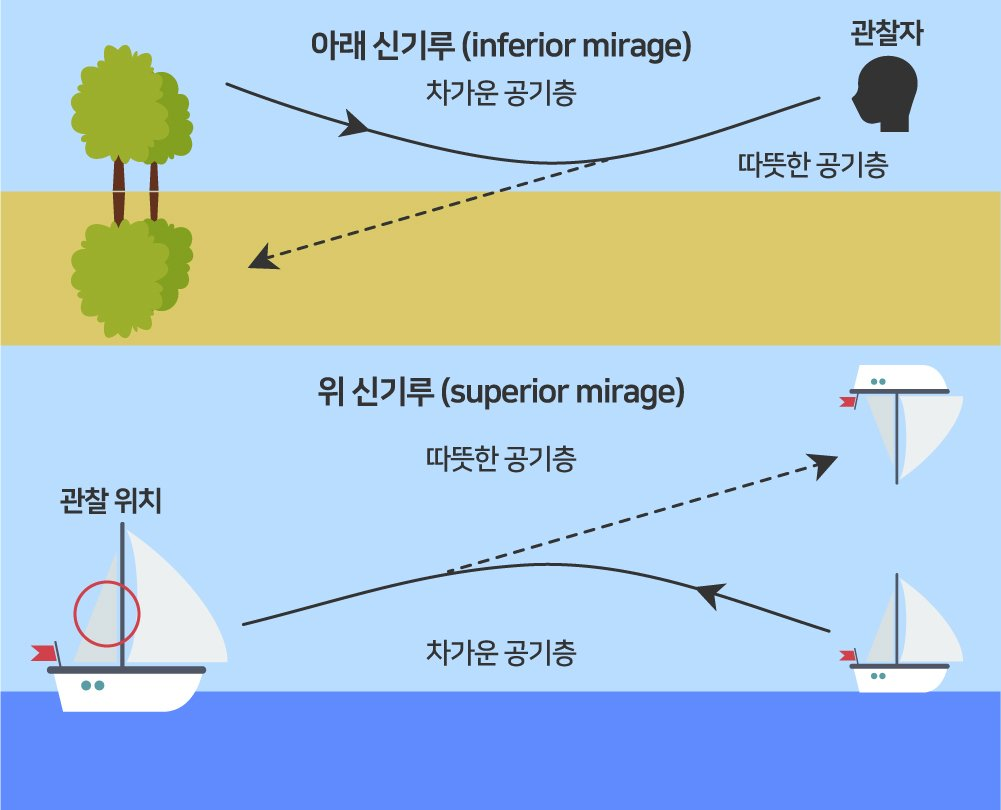
\includegraphics[width=\textwidth]{images/mirage_2-100.jpg}
			\end{figure}
		\end{minipage}	
		&
		\begin{minipage}[t]{0.45\textwidth} \scriptsize	
			\questionset {빛이 따뜻한 공기에서 찬 공기로 진행할 때 그 경로는 곡선이다. 빛은 어느 쪽으로 휘며 그 이유는 무엇인가?}
			\solutionset {
					빛은 밀도가 높을수록 굴절률이 커져(속도가 감소되어) 밀도가 큰 쪽으로 휘게 된다. 따라서 빛은 찬 공기 쪽으로 휘게 된다.
					}

		\end{minipage}
	\end{tabular}
\end{frame}

\begin{frame}[t]{아래 신기루(inferior mirage)}
	\begin{tabular}{ll}
		\begin{minipage}[t]{0.6\textwidth}\scriptsize
			\begin{figure}[t]
				\includegraphics[trim=300 50 50 500, clip, 
				page=482, width=\textwidth]{\bookfile}
			\end{figure}
		\end{minipage}	
		&
		\begin{minipage}[t]{0.35\textwidth} \scriptsize	
			\questionset {아래 신기루(inferior mirage)는 어떻게 나타나는가?}
			\solutionset {
				사막과 같이 지표가 가열된 경우 위쪽보다 아래쪽의 밀도가 낮다. 이러한 경우 빛은 밀도가 높은 쪽으로 휘게 된다. 따라서 물체로부터 나온 빛이 지구의 곡률과 반대방향으로 휘어 우리 눈에 들어오게 된다. 우리는 물체가 마치 아래 쪽에 있는 것처럼 자각하게 되는데, 대상의 실제 위치 아래쪽에 상이 보인다는 의미에서 아래 신기루라고 한다.
				전형적인 사막의 신기루에서 나타나는 야자수 주변의 물은 사실 하늘에서 진행한 빛이 아래로 볼록하게 굴절되어 만들어지는 상으로, 야자수는 실제이지만 물과 반사된 야자수는 신기루의 일부이다				
					}

		\end{minipage}
	\end{tabular}
\end{frame}

\begin{frame}[t]{아래 신기루(inferior mirage)}
	\begin{tabular}{ll}
		\begin{minipage}[t]{0.4\textwidth}\scriptsize
			\begin{figure}[t]
				\includegraphics[trim=300 50 50 500, clip, 
				page=482, width=\textwidth]{\bookfile}
			\end{figure}
		\end{minipage}	
		&
		\begin{minipage}[t]{0.55\textwidth} \scriptsize	
			\questionset {아래 신기루는 종종 상이 뒤집혀서 보인다. 그 이유를 설명하시오.}
			\solutionset {
				나무 꼭대기 근처를 통과한 빛이 나무 밑 근처를 통과한 빛보다 더 굴절되기 때문에 상이 뒤집혀서 보일 수 있다. 
				그러나 신기루가 발생했을 때 항상 상이 뒤집히는 것은 아니다. \\
				\begin{figure}[t]
					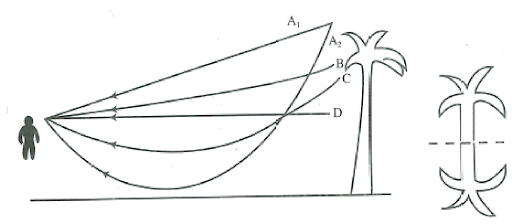
\includegraphics[width=\textwidth]{images/reverse.png}
				\end{figure}
					}

		\end{minipage}
	\end{tabular}
\end{frame}

\begin{frame}[t]{상층 신기루(superior mirage)}
	\begin{tabular}{ll}
		\begin{minipage}[t]{0.6\textwidth}\scriptsize
			\begin{figure}[t]
				\includegraphics[trim=35 35 160 580, clip, 
				page=483, width=\textwidth]{\bookfile}
			\end{figure}
		\end{minipage}	
		&
		\begin{minipage}[t]{0.35\textwidth} \scriptsize	
			\questionset {상층 신기루는 어떻게 나타나는가?.}
			\solutionset {
				한대 지역이나 찬 해양 표면 위에서는 지표 근처 또는 해양 근처의 온도가 바로 위의 공기보다 훨씬 더 냉각되어 상층보다 밀도가 매우 높을 때가 있다. 이럴 경우 빛은 찬 공기 쪽으로 휘게 되고 사막 신기루와는 반대로 상이 위쪽에 보이도록 한다.\\
				그림처럼 시야에서 사라진 배를 볼수 있게 되는 경우를 떠오름(looming) 이라고도 한다.
					}
		\end{minipage}
	\end{tabular}
\end{frame}


\begin{frame}[t]{파타 모르가나(Fata Morgana)}
	\begin{tabular}{ll}
		\begin{minipage}[t]{0.6\textwidth}\scriptsize
			\begin{figure}[t]
				\includegraphics[trim=350 540 40 50, clip, 
				page=484, width=\textwidth]{\bookfile}
			\end{figure}
		\end{minipage}	
		&
		\begin{minipage}[t]{0.35\textwidth} \scriptsize	
			\questionset {파타 모르가나가 관측되는 원리를 설명하시오.}
			\solutionset {
				큰 온도 차이가 발생하는 연안 지역에서 자주 관측되는 것으로 지표면 근처의 물체를 길게 보이게 하는 길어보임(towering)의 한 종류이며, 왼쪽 이미지에서 위쪽 부분은 신기루로 빙산이 역전된 상이다.
					}
		\end{minipage}
	\end{tabular}
\end{frame}



\begin{frame}[t]{신기루}
	\begin{tabular}{ll}
		\begin{minipage}[t]{0.55\textwidth}\scriptsize
			\begin{figure}[t]
				\includegraphics[trim=30 390 355 205, clip, 
				page=483, width=\textwidth]{\bookfile}
			\end{figure}
		\end{minipage}	
		&
		\begin{minipage}[t]{0.4\textwidth} \scriptsize	
			\questionset {신기루는 왜 관찰자가 가까이 접근하면 항상 사라질까?}
			\solutionset {
					신기루는 지표면 근처의 기온 변화로 인한 공기의 밀도 변화로 나타나는 것이다. 
					즉 물체로부터 반사된 빛이 일정한 경로를 휘어져 관측자에 들어오기 때문에 나타나는데, 관찰자가 신기루에 가까이 접근하면 빛이 휠 수 있는 충분한 거리가 확보되지 않으므로 사라지게 된다.
					}

		\end{minipage}
	\end{tabular}
\end{frame}



\section{무지개}

\begin{frame}[t]{빛의 분산}
	\begin{tabular}{ll}
		\begin{minipage}[t]{0.9\textwidth}\scriptsize
			\begin{figure}[t]
				\includegraphics[trim=50 20 50 650, clip, 
				page=485, width=\textwidth]{\bookfile}
			\end{figure}
		\end{minipage}	
		&
		\begin{minipage}[t]{0.05\textwidth} \scriptsize	

		\end{minipage}
	\end{tabular}
	
	\scriptsize
	빛의 색(파장)에 따라 굴절되는 각도가 조금씩 다름.
			보라색은 속도가 가장 느려 굴절이 많이 일어나며, 붉은색은 속도가 가장 빨라 굴절이 가장 적게 일어 남.
			태양빛이 물로 입사하면 파장별로 서로 다른 굴절 효과가 속도에 따라 태양빛을 분리함. 이와 같이 굴절에 의해 색이 분리되는 것을 분산(dispersion)이라고 함.
\end{frame}


\begin{frame}[t]{1차 무지개}
	\begin{tabular}{ll}
		\begin{minipage}[t]{0.5\textwidth}\scriptsize
			\begin{figure}[t]
				\includegraphics[trim=0 410 230 0, clip, 
				page=485, width=\textwidth]{\bookfile}
			\end{figure}
		\end{minipage}	
		&
		\begin{minipage}[t]{0.45\textwidth} \scriptsize	
			\questionset {1차 무지개가 생성되는 원리를 설명하시오.}
			\solutionset {
				1차 무지개는 물방울에서의 빛의 분산으로 인해 나타난다. 
				태양빛이 물방울로 입사하면 공기-물방울 경계면에서 한 번 굴절이 되고 물방울-공기 경계면에서 한 번 반사가 된 후, 물방울-공기 경계면에서 굴절이 되어 빠져나간다. 
				이 과정에서 빛은 파장별로 분산이 되는데 입사하는 태양 빛과 무지개를 구성하는 분산된 색 사이의 각은 빨간색이 42°이고 보라색이 40°이다. 그래서 되돌아온 빛은 보라색이 위쪽, 붉은색이 아래쪽에 위치한다. 
				그러므로 어떤 한 빗방울에 대해서 관측자는 오직 한 가지 색만 볼 수 있다. 
					}

		\end{minipage}
	\end{tabular}
\end{frame}


\begin{frame}[t]{1차 무지개}
	\begin{tabular}{ll}
		\begin{minipage}[t]{0.9\textwidth}\scriptsize
			\begin{figure}[t]
				\includegraphics[trim=50 420 50 55, clip, 
				page=486, width=0.85\textwidth]{\bookfile}
			\end{figure}
		\end{minipage}	
		&
		\begin{minipage}[t]{0.05\textwidth} \scriptsize	
			

		\end{minipage}
	\end{tabular}
		\scriptsize
		특정 위치의 관측자는 서로 다른 위치에 있는 여러 물방울로부터 되돌아온 다양한 파장의 빛을 보게 된다.\\
		즉, 수없이 많은 물방울로부터 빛이 분산되므로, 관측자의 위치에 어떤 물방울에 의해 분산된 적색의 빛이 들어왔다면 그보다 아랫쪽 물방울로부터 적색보다 파장이 조금 더 짧은 빛이 들어오고, 더 아랫쪽 물방울로부터는 그 파장보다 조금 더 짧은 빛이 들어오게 된다. 
		따라서 1차 무지개는 위에서부터 아래로 빨강~보라의 순서가 된다.

\end{frame}


\begin{frame}[t]{2차 무지개}
	\begin{tabular}{ll}
		\begin{minipage}[t]{0.5\textwidth}\scriptsize
			\begin{figure}[t]
				\includegraphics[trim=300 30 30 540, clip, 
				page=486, width=\textwidth]{\bookfile}
			\end{figure}
		\end{minipage}	
		&
		\begin{minipage}[t]{0.45\textwidth} \scriptsize	
			\begin{itemize}
				\item 2차 무지개 역시 물방울에서의 빛의 분산으로 인해 나타난다. 
				\item 1차 무지개와의 차이는 물방울 내부에서 반사가 2번 일어나게 된다는 점이다.
				\item 추가된 반사에 의해 보통 붉은 빛은 입사광선과 $50\rm^{\circ}$의 각을 이루게 되며, 보라색 빛은 $50\rm^{\circ}$보다 더 큰 각을 이루게 된다.
				\item 그래서 되돌아온 빛은 보라색이 아래쪽, 빨간색이 위쪽에 위치한다. 
			\end{itemize}

			\questionset{일반적으로 1차 무지개가 2차 무지개보다 흐린 이유를 설명하시오.}
			\solutionset{
				빛이 물방울 표면 안쪽에 닿을 때마다 일부의 빛은 반사되지만, 
				나머지는 반사하는 표면을 투과하여 무지개 형성에 무관하다. 
				그래서 2차 무지개는 항상 형성되지만 1차 무지개보다 흐리고 관측이 안되는 경우도 있다. 
			}


		\end{minipage}
	\end{tabular}
		

\end{frame}

\begin{frame}[t]{무지개}
	\begin{tabular}{ll}
		\begin{minipage}[t]{0.6\textwidth}\scriptsize
			\begin{figure}[t]
				\includegraphics[trim=0 410 50 0, clip, 
				page=487, width=\textwidth]{\bookfile}
			\end{figure}
		\end{minipage}	
		&
		\begin{minipage}[t]{0.35\textwidth} \scriptsize	
			\begin{itemize}
				\item 그런데 1차 무지개와 마찬가지로 관측자는 다양한 위치에서 되돌아온 다양한 파장의 빛을 보게 된다.  
				\item 다만 하나의 물방울로부터 되돌아온 빛의 순서가 1차 무지개와는 반대이다. 즉, 위쪽에 있는 물방울이 파장이 조금 짧은 빛(입사광선과 이루는 각이 큰)을 시선 방향으로 보내기 때문에 2차 무지개는 아래서부터 위로 빨강~보라 순서로 나타나게 된다. 
			\end{itemize}

		\end{minipage}
	\end{tabular}
\end{frame}


\begin{frame}[t]{무지개}
	\begin{figure}[t]
		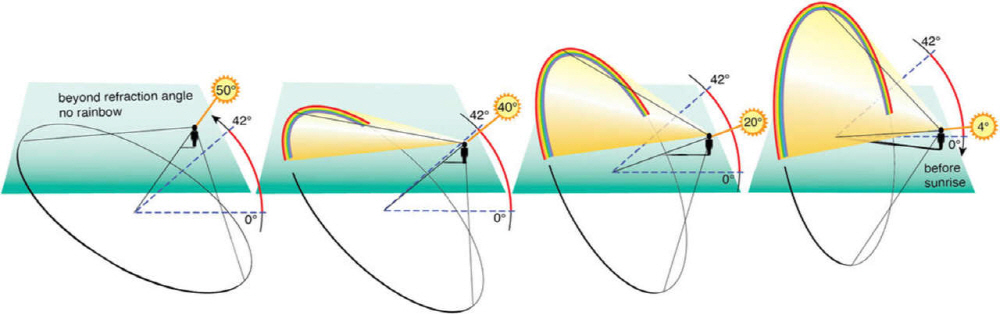
\includegraphics[width=0.9\textwidth]{images/rainbow_42.jpg}
	\end{figure}

	\begin{tabular}{ll}
		\begin{minipage}[t]{0.475\textwidth}\scriptsize
			\questionset {아침에 무지개를 찾는다면 어떤 방향에서 찾아야 하는지 그 이유를 설명하고, 구전에 따라 앞으로의 날씨를 예측 하시오.}
			\solutionset {		
				아침에는 태양이 동쪽에 있으므로, 무지개를 찾으려면 서쪽 방향을 보아야 한다. 서쪽에서 비가 내리고 있거나 공기 중에 물방울이 있다면 무지개를 볼 수 있을 것이다.
				그러므로 아침의 무지개는 우리나라에 비가 내리거나 날이 흐릴 것이라는 것을 예측하게 한다. \\
					}

		\end{minipage}	
		&
		\begin{minipage}[t]{0.475\textwidth} \scriptsize	
			\questionset {하짓날 정오에 수원($37.5\rm^{\circ}N$)에서 무지개를 관찰할 수 있을까?}
			\solutionset {		
				하짓날 정오에 태양의 고도는 $90\rm^{\circ} - 37.5\rm^{\circ} + 23.5\rm^{\circ} = 76\rm^{\circ}$이다. \\
				무지개는 태양빛이 관측자와 $42\rm^{\circ}$의 각을 이룰 때 생기므로, 태양의 고도가 $42\rm^{\circ}$보다 높을 경우 무지개를 볼 수 없다.
					}
		\end{minipage}
	\end{tabular}
\end{frame}




\section{무리, 무리해, 해기둥}


\begin{frame}[t]{무리(halos)}
	\begin{tabular}{ll}
		\begin{minipage}[t]{0.475\textwidth}\scriptsize
			\begin{figure}[t]
				\includegraphics[trim=0 480 280 0, clip, 
				page=488, width=\textwidth]{\bookfile}
			\end{figure}
			\scriptsize
			무리는 태양이나 달을 중심으로 큰 지름을 가지는 좁고 하얀  고리로 나타난다. 
		\end{minipage}	
		&
		\begin{minipage}[t]{0.475\textwidth} \scriptsize	
			\begin{figure}[t]
				\includegraphics[trim=50 30 350 480, clip, 
				page=488, width=0.85\textwidth]{\bookfile}
			\end{figure}
			\scriptsize
			네가기 기본 유형의 빙정들 (A: 판상, B: 기둥, C: 모자 쓴 기둥, D: 탄환)
		\end{minipage}
	\end{tabular}
\end{frame}



\begin{frame}[t]{무리(halos)}
	\begin{tabular}{ll}
		\begin{minipage}[t]{0.4\textwidth}\scriptsize
			\begin{figure}[t]
				\includegraphics[trim=390 280 50 60, clip, 
				page=488, width=0.7\textwidth]{\bookfile}
			\end{figure}
		\end{minipage}	
		&
		\begin{minipage}[t]{0.55\textwidth} \scriptsize	
			\questionset {무리의 형성과정을 설명하시오.}
			\solutionset {		
				무리는 빙정에 의한 태양빛의 분산에 의해 만들어진다. 보통 권운을 형성하는 빙정이 무작위 방향성을 가질 때 6면체 빙정들이 이루는 각으로 인해 한 면에 빛이 입사하면 빛은 진행방향의 $22\rm^{\circ}$나 $46\rm^{\circ}$ 방향으로 빛을 집중적으로 굴절시킨다. \\
				$22\rm^{\circ}$ 무리는 빙정의 상부나 하부가 아닌 옆면으로 입사한 태양이나 달빛의 대부분이 맞은편 면으로 나올때 생성된다.  \\
				$46\rm^{\circ}$ 무리는 빙정의 상부나 하부가 아닌 옆면으로 입사한 후 빙정의 상부나 하부로 나올때 생성된다. 
				
				\begin{figure}[t]
					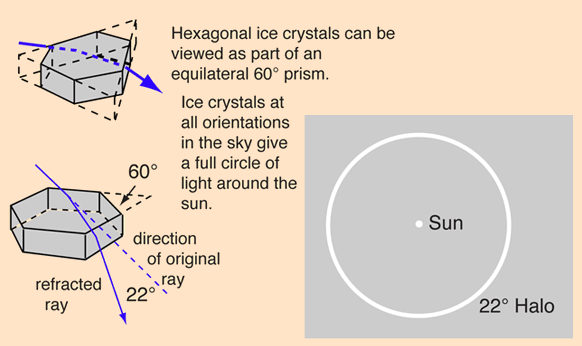
\includegraphics[width=0.75\textwidth]{images/halo22.png}
				\end{figure}	
				}

		\end{minipage}
	\end{tabular}
\end{frame}

\begin{frame}[t]{무리(halos)}
	\begin{tabular}{ll}
		\begin{minipage}[t]{0.475\textwidth}\scriptsize
			\questionset {무리의 색깔 배열은 어떻게 나타나는가?}
			\solutionset {		
				무지개와 마찬가지로 관찰자의 입장에서 보면, 어떤 빙정에 의해 분산된 적색의 빛이 들어왔다면 그 옆의 빙정으로부터 적색보다 파장이 조금 더 짧은 빛이 들어오고, 더 옆의 빙정으로부터는 그 파장보다 조금 더 짧은 빛이 들어온다. 그래서 결국 안쪽이 붉은색, 바깥쪽이 보라색으로 나타난다. 
				물방울에 비해서 빙정은 모양이 불규칙하고 크기가 커서 분리된 색이 서로 겹치기 때문에, 무지개처럼 색이 분리되어 보이지 않고 흰색으로 보이는 경우가 많다.\\
					}
		\end{minipage}	
		&
		\begin{minipage}[t]{0.475\textwidth} \scriptsize	
			\questionset {무리와 무지개의 공통점과 차이점을 설명하시오.}
			\solutionset {		
				공통점: 두 현상 모두 빛의 분산으로 인해 나타나는 현상이다. 
				차이점:\\
				 - 무리는 빙정에서, 무지개는 물방울에서 나타나는 현상이다. \\
				 - 무지개는 무리 보다 훨씬 크고 분명한 색을 띈다.\\
				 - 무리는 전방 산란이지만, 무지개는 후방 산란이다.
					}
		\end{minipage}
	\end{tabular}
\end{frame}

\begin{frame}[t]{무리해 (sun dogs or parhelia)}
	\begin{tabular}{ll}
		\begin{minipage}[t]{0.5\textwidth}\scriptsize
			\begin{figure}[t]
				\includegraphics[trim=40 220 330 370, clip, 
				page=490, width=\textwidth]{\bookfile}
			\end{figure}
			\scriptsize	
			지평선 부근에 태양이 있을 때 연직 방향으로 배열된 상당수의 빙정이 천천히 하강할 때 태양 양쪽 $22^{\circ}$ 각거리 위치에 두 개의 밝은 지역이 나타나는 현상을 무리해라고 한다. \\
			무리해 역시 무리와 같이 빙정에 의한 태양빛의 분산에 의해 만들어진다.
		\end{minipage}	
		&
		\begin{minipage}[t]{0.45\textwidth} \scriptsize	\
			\questionset {무리를 발생시키는 빙정과 무리해를 발생시키는 빙정은 방향성에 있어서 어떠한 차이를 가지고 있는가?}
			\solutionset {		
				무리를 만드는 빙정은 일반적으로 무작위의 방향성을 띈다. 반면 무리해를 만드는 빙정은 장축이 수직방향으로 배열되어야 한다.
				\begin{figure}[t]
					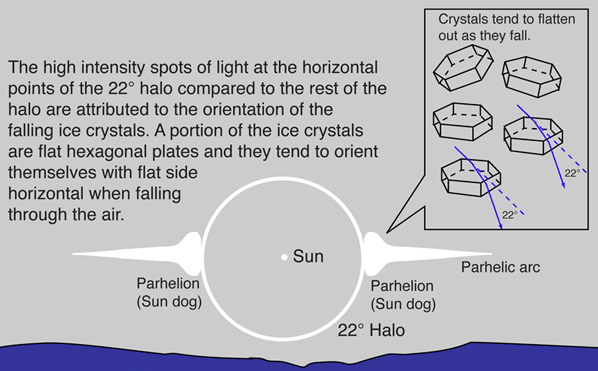
\includegraphics[width=\textwidth]{images/sundog.png}
				\end{figure}		
				}

		\end{minipage}
	\end{tabular}
\end{frame}


\begin{frame}[t]{해기둥 (sun pillar)}
	\begin{tabular}{ll}
		\begin{minipage}[t]{0.5\textwidth}\scriptsize
			\begin{figure}[t]
				\includegraphics[trim=350 520 0 0, clip, 
				page=490, width=\textwidth]{\bookfile}
			\end{figure}
		\end{minipage}	
		&
		\begin{minipage}[t]{0.45\textwidth} \scriptsize	
			\questionset {해기둥은 어떻게 형성되는가?}
			\solutionset {		
				판상 모양의 빙정들 하부에서 반사된 빛이 관측자에게 도달할 때 관측됨. 보통 일몰 직전이나 일출 직후 광선들이 태양으로부터 위로 뻗쳐 나갈 때 자주 보임.
				\begin{figure}[t]
					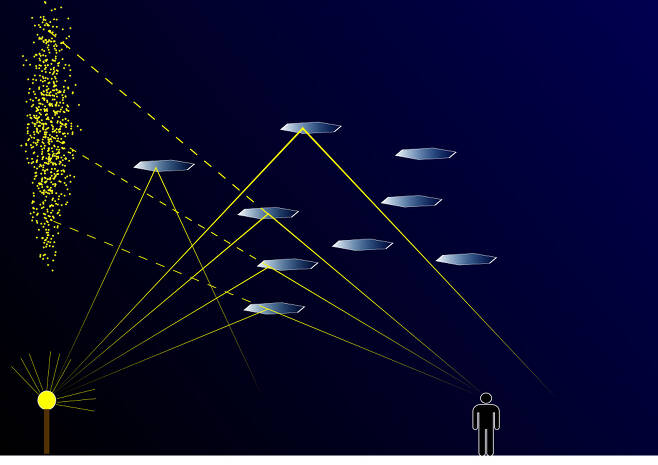
\includegraphics[width=\textwidth]{images/pillar.jpg}
				\end{figure}
				}
		\end{minipage}
	\end{tabular}
\end{frame}


\begin{frame}[t]{광륜(glory)}
	\begin{tabular}{ll}
		\begin{minipage}[t]{0.4\textwidth}\scriptsize
			\begin{figure}[t]
				\includegraphics[trim=45 50 320 360, clip, 
				page=489, width=\textwidth]{\bookfile}
			\end{figure}
		\end{minipage}	
		&
		\begin{minipage}[t]{0.55\textwidth} \scriptsize	
			\questionset {광륜이란 무엇이며 이러한 이름이 붙게 된 기원은 무엇인가?}
			\solutionset {		
				광륜이란 구름이나 안개 위에 투영된 그림자 주위에 무지개와 같이 한 가지 또는 그 이상의 색을 가진 고리 모양이 보이는 것이다. 
				안개 위로 투영된 관찰자 머리의 그림자 주위에 나타날 수 있어서 glory라는 이름이 붙었다.\\

				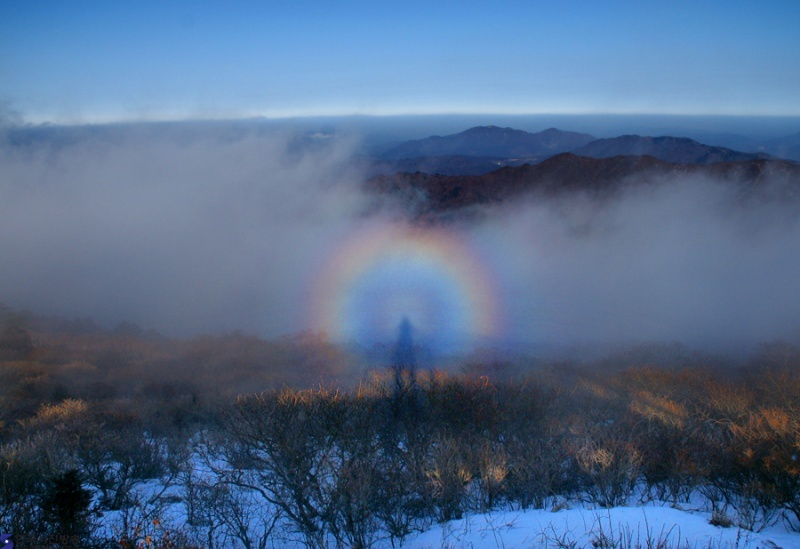
\includegraphics[width=0.85\textwidth]{images/1328771964-23.jpg}
				}
		\end{minipage}
	\end{tabular}
\end{frame}


\begin{frame}[t]{광륜(glory)}
	\begin{tabular}{ll}
		\begin{minipage}[t]{0.4\textwidth}\scriptsize
			\begin{figure}[t]
				\includegraphics[trim=400 415 55 90, clip, 
				page=489, width=\textwidth]{\bookfile}
			\end{figure}
		\end{minipage}	
		&
		\begin{minipage}[t]{0.55\textwidth} \scriptsize	
			\questionset {광륜의 형성과정을 설명하시오.}
			\solutionset {		
				광륜이 어떻게 형성되는가에 대한 과학적 설명을 아직 논란중에 있다. \\
				하나의 가설은 광륜은 무지개처럼 물방울에 의해 발생하지만, 상대적으로 크기가 매우 작고 균일한 크기의 물방울에서 발생한다. 
				입사한 광선이 굴절되고 내부적으로 반사가 일어난 뒤, 입사한 반대면으로 빠져나올 때 회절이 발생하여 형성되는 것으로 보여짐. 
				광륜이 형성되기 위해서는 태양광선이 태양쪽으로 후방 산란될 수 있도록 $180^{\circ}$ 휘어져야 하는데, 회절이 발생하면 이러한 추가적 휘어짐 발생이 가능하다. 

				광륜은 언제나 태양의 반대쪽에 형성되므로 관측자의 그림자는 항상 광륜 안에서 발견된다. 
				독일의 브로켄 산에서 자주 관측되어 브로켄 현상(Brocken spectre)이라고도 한다.
				}
		\end{minipage}
	\end{tabular}
\end{frame}

% \begin{frame}[t]{광륜(glory)}
% 	\begin{tabular}{ll}
% 		\begin{minipage}[t]{0.6\textwidth}\scriptsize
% 			\begin{figure}[t]
% 				\includegraphics[trim=400 550 50 40, clip, 
% 				page=489, width=\textwidth]{\bookfile}
% 			\end{figure}
% 		\end{minipage}	
% 		&
% 		\begin{minipage}[t]{0.35\textwidth} \scriptsize	
% 			\questionset {광륜의 색깔 배열을 설명하시오.}
% 			\solutionset {		
% 				광륜은 회절이 발생하는 것만 제외하면 1차 무지개와 형성과정이 유사하다. 그래서 하나의 물방울에서 되돌아온 빛은 보라색이 위쪽, 붉은색이 아래쪽에 위치한다. 
% 				그러나 수없이 많은 물방울로부터 빛이 분산되므로, 관측자의 위치에 어떤 물방울에 의해 분산된 적색의 빛이 들어왔다면 그보다 아랫쪽 물방울로부터 더 짧은 파장의 빛이 들어온다. 
% 				그러므로 광륜은 안쪽이 보라색, 바깥쪽이 적색으로 배열된다. 
% 				}
% 		\end{minipage}
% 	\end{tabular}
% \end{frame}



\begin{frame}[t]{광환(corona)}
	\begin{tabular}{ll}
		\begin{minipage}[t]{0.6\textwidth}\scriptsize
			\begin{figure}[t]
				\includegraphics[trim=40 40 250 440, clip, 
				page=491, width=\textwidth]{\bookfile}
			\end{figure}
		\end{minipage}	
		&
		\begin{minipage}[t]{0.35\textwidth} \scriptsize	
			\questionset {광환의 색은 어떻게 나타나며 무리와의 차이점은?}
			\solutionset {		
				광환의 색은 구름을 구성하는 작고 균일한 물방울이나 빙정에 의해 햇빛이나 달빛이 회절이 일어나고 회절된 빛이 간섭할 때 나타난다. \\
				광환은 바깥쪽이 붉은색이고 안쪽이 파란색을 띤 흰색임에 반해 무리는 색깔 배열이 반대이다.
				또한 광환은 무리($22^{\circ}$)보다 발광체에 근접하여 형성됨
				}
		\end{minipage}
	\end{tabular}
\end{frame}




\begin{frame}[t]{광환(corona)}
	\begin{tabular}{ll}
		\begin{minipage}[t]{0.6\textwidth}\scriptsize
			\begin{figure}[t]
				\includegraphics[trim=40 40 250 440, clip, 
				page=491, width=\textwidth]{\bookfile}
			\end{figure}
		\end{minipage}	
		&
		\begin{minipage}[t]{0.35\textwidth} \scriptsize	
			\questionset {광환의 색은 어떻게 나타나며 무리와의 차이점은?}
			\solutionset {		
				광환의 색은 구름을 구성하는 작고 균일한 물방울이나 빙정에 의해 햇빛이나 달빛이 회절이 일어나고 회절된 빛이 간섭할 때 나타난다. 
				광환은 바깥쪽이 붉은색이고 안쪽이 파란색을 띤 흰색임에 반해 무리는 색깔 배열이 반대이다.
				또한 광환은 무리($22^{\circ}$)보다 발광체에 근접하여 형성됨
				}
		\end{minipage}
	\end{tabular}
\end{frame}




\begin{frame}[t]{채운 (iridescent clouds)}
	\begin{tabular}{ll}
		\begin{minipage}[t]{0.45\textwidth}\scriptsize
			\begin{figure}[t]
				\includegraphics[trim=330 510 50 50, clip, 
				page=491, width=\textwidth]{\bookfile}
			\end{figure}
		\end{minipage}	
		&
		\begin{minipage}[t]{0.5\textwidth} \scriptsize	
			채운은 고층원, 권적운 또는 렌즈운 등에 의해 발행하며 일반적으로 보라색, 분홍색, 녹색과 같은 밝은 색의 영역으로 나타나는데, 구름 가장자리에서 보인다. \\

			\questionset {채운은 어떻게 형성되며, 관측하기 위한 최적의 시간은?}
			\solutionset {		
				채운과 관련된 색의 발현은 작고 균질한 빙정, 구름방울에 의한 달빛 또는 태양빛의 회절에 의해 형성된다.
				채운은 태양이 구름 뒤에 있거나 태양이 빌딩이나 지형학적 장애물 뒤로 가려진 직후에 관측하기 좋다.
				}
		\end{minipage}
	\end{tabular}
\end{frame}




